\q{12}{Boba Distributions}

Anna is curious about her boba spending habits. The following is a histogram of her weekly spending on boba, over the span of \textbf{50} weeks (she doesn’t drink boba on her yearly two week vacation): 
%FIXME Do we like placement of hist? 
\begin{center}
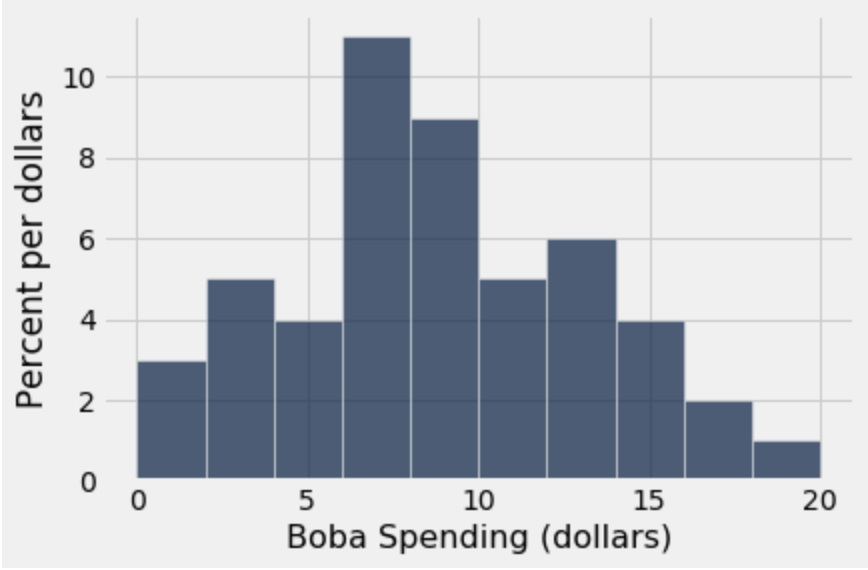
\includegraphics[scale=.6]{q3_boba}
\end{center}
The spending is divided into bins of width 2: [0,2), [2,4) ... [18,20).  

Assume that all of the data is shown on the histogram (Anna never spent \$20 or more in a given week).  

For the following questions, write a \textbf{mathematical expression} for the answer, or write \textit{“Not possible”} if it is not possible to calculate the desired quantity with the information in the given histogram.

\begin{enumerate}
\vskip .2in
% Do we want to bold percent? 
\subq{3} In what percent of weeks did Anna spend \$16 or more on boba?

\solution{2*2 + 1*2 = 6\%}

\vskip .6in
% Do we want to bold percent? 
\subq{3} In what percent of weeks did Anna spend between \$12 and \$15 on boba? 

\solution{Not possible to determine}

\vskip .6in
\subq{3} During how many weeks did Anna spend between \$10 and \$13 dollars?

\vskip 0.1in
\begin{tabular}{l@{\hskip 1in}l@{\hskip 1in}l@{\hskip 1in}l}
\bubble\quad 11 weeks \\
\solutionbubble \quad Between 5 and 11 weeks \\
\bubble \quad 22 weeks \\
\bubble \quad Between 10 and 22 weeks \\
\bubble \quad Not possible to calculate using the histogram
\end{tabular}

\vskip .2in
\subq{3} After looking over her notes, Anna finds that she entered the wrong data for two of the weeks when constructing the histogram. She is not sure whether her spending in those weeks should go in the [12, 14) or [14, 16) bin, so she decides to combine all of the data in those two bins into one bin of width 4, from [12,16). What is the height of this new bin? 

\solution{(0.6*2 + 0.4*2)/4 = 5 \%/\$}


\end{enumerate}
